\documentclass{article}
\usepackage[T1]{fontenc}
\usepackage[utf8]{inputenc}
\usepackage[submission]{ismir}
\usepackage{amsmath,cite,url}
\usepackage{graphicx}
\usepackage{booktabs}
\usepackage{color}

\title{A Symbolic Music-Theory Benchmark for Computational Musicology and LLM Evaluation}

\oneauthor
  {Anonymous Authors}
  {Anonymous Affiliations\\\texttt{anonymous@ismir.net}}

\def\authorname{Anonymous Authors}

\sloppy

\begin{document}

\maketitle

\begin{abstract}
We present a symbolic benchmark for evaluating whether large language models can identify, manipulate, and explain core music-theoretical structures. The benchmark contains eight zero-shot tasks spanning interval identification, chord identification, harmonic-function classification, transposition, melodic inversion, retrograde, rhythmic scaling, and voice-leading violation detection. We organize these tasks into two output families: label classification and note-sequence transformation. The benchmark is designed around automatically verifiable symbolic inputs and outputs, with task-specific metrics and a unified evaluation pipeline. In addition to the standard benchmark mode, which prioritizes strict reproducibility, we introduce an optional explanation layer that supports qualitative analysis of musicological reasoning without affecting the main score. We frame the current release as a deliberately constrained V1 scope: harmonic function is limited to major mode, voice-leading is simplified to two voices, and harmonic vocabulary is reduced to a stable subset of tonal sonorities. This design enables reproducible evaluation today while leaving space for future expansions in analytical coverage. The resulting benchmark is intended both as an engineering artifact for model comparison and as a computational musicology instrument for studying the gap between structural correctness and analytical explanation.
\end{abstract}

\section{Introduction}
\label{sec:introduction}

Recent work in symbolic music modeling has improved tokenization, generation, and pretraining strategies, but benchmark design for \emph{music-theoretical reasoning} remains underdeveloped. Many symbolic systems can generate convincing musical continuations, yet it is often unclear whether they can reliably identify analytical categories such as harmonic function, or apply explicit transformational rules such as inversion and retrograde under controlled conditions.

This paper introduces a symbolic benchmark centered on a simple question: \emph{can language models correctly capture and manipulate core music-theoretical structures, and does structural correctness align with meaningful analytical reasoning?} The benchmark focuses on symbolic input rather than audio so that ground truth can be generated and verified with rule-based logic. This choice does not claim that audio is unimportant; rather, it provides a controlled first step toward reproducible evaluation.

Our contribution has three parts. First, we operationalize foundational concepts from music theory as benchmark tasks with stable input-output contracts. Second, we provide a multi-task evaluation pipeline that supports both label prediction and note-sequence transformation under a shared interface. Third, we separate formal correctness from analytical explanation through an optional explanation layer, allowing the benchmark to support both strict evaluation and musicology-facing qualitative analysis.

\section{Related Work}
\label{sec:related_work}

Symbolic music research has produced strong representational and modeling frameworks, including event-based tokenizations such as REMI and pretrained symbolic models such as MusicBERT \cite{huang2020pop, huang2021musicbert}. These systems have broadened the scope of symbolic music generation and understanding, but much of the evaluation still emphasizes generation quality, continuation quality, or downstream predictive performance rather than direct assessment of music-theoretical reasoning.

More broadly, recent language-model evaluation research has emphasized benchmark design, structured outputs, and reproducibility \cite{liang2023holistic}. Our work brings that benchmarking perspective into symbolic music reasoning by defining tasks that remain close to recognizable analytical concepts from music theory while still being machine-checkable.

The proposed benchmark is therefore not a new symbolic representation model. Instead, it is an evaluation resource intended to support comparison across models, tokenizers, and prompting conditions, while also enabling discussion of what counts as musical understanding in a symbolic setting.

\section{Benchmark Design}
\label{sec:benchmark_design}

\subsection{Task Families}

The benchmark contains eight tasks organized into two output families. Label classification tasks require the model to predict a single symbolic label:
\begin{itemize}
    \item interval identification,
    \item chord identification,
    \item harmonic-function classification,
    \item voice-leading violation detection.
\end{itemize}

Sequence transformation tasks require the model to generate a transformed note sequence:
\begin{itemize}
    \item transposition,
    \item melodic inversion,
    \item retrograde,
    \item rhythmic augmentation or diminution.
\end{itemize}

The benchmark uses a canonical prediction interface. Label tasks return \texttt{prediction\_label}; sequence tasks return \texttt{prediction\_notes}; and an optional \texttt{prediction\_explanation} field can be added for qualitative analytical output without affecting the primary metric.

\subsection{Representations and Views}

Each benchmark case is produced in a raw note-level representation and then exported into multiple tokenizer views, including \texttt{note\_level}, \texttt{midilike}, and \texttt{remilike}. These alternative views allow us to ask whether representational choices influence benchmark performance, rather than treating symbolic input as a single fixed format.

\subsection{Current V1 Scope}

We intentionally frame the current benchmark as a V1 scope rather than as full tonal coverage. Harmonic function is limited to major mode with the three coarse classes \texttt{tonic}, \texttt{predominant}, and \texttt{dominant}. Voice-leading is simplified to a two-voice setting with labels \texttt{parallel\_fifths}, \texttt{voice\_crossing}, and \texttt{none}. Chord identification uses a reduced vocabulary focused on major, minor, diminished, augmented, and dominant-seventh sonorities.

These simplifications are methodological rather than theoretical claims about music itself. They narrow the benchmark enough to keep generation, prompting, decoding, and evaluation stable, while still supporting meaningful analytical discussion.

\begin{figure}[t]
  \centering
  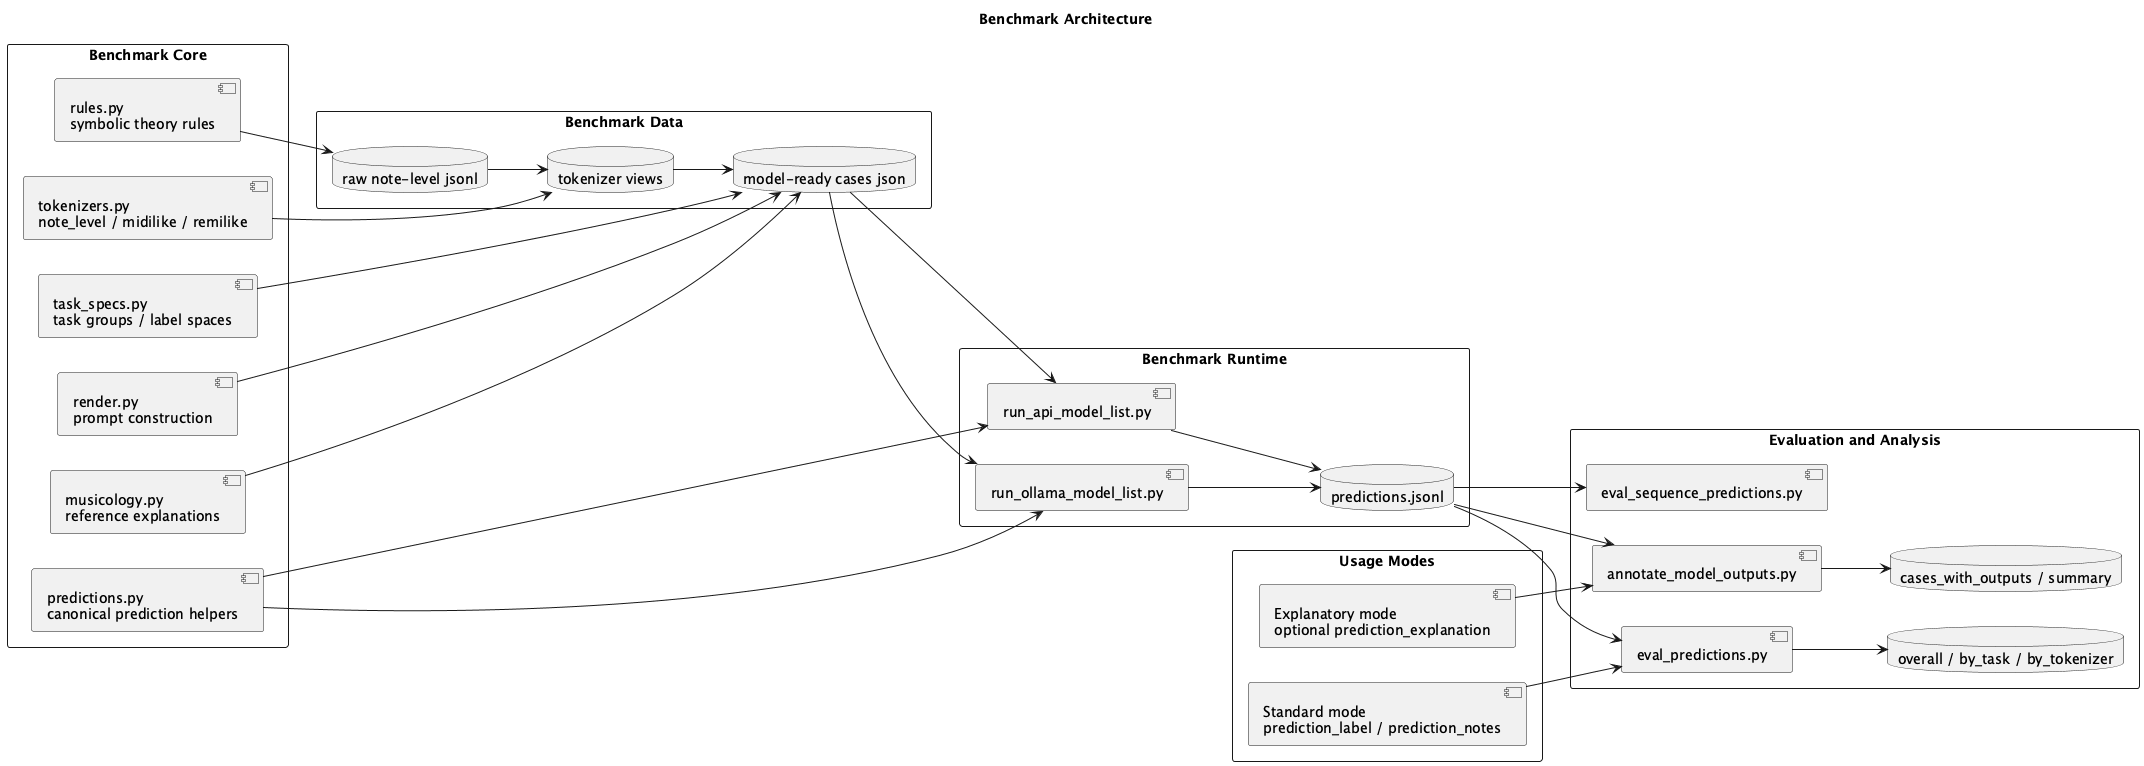
\includegraphics[width=\columnwidth]{figures/benchmark-architecture.png}
  \caption{High-level architecture of the benchmark pipeline, separating theory logic, representation, execution, and analysis.}
  \label{fig:architecture}
\end{figure}

\section{Pipeline and Reproducibility}
\label{sec:pipeline}

The benchmark is implemented as a rule-based pipeline. A generator produces canonical cases at the raw symbolic level. These are then exported to tokenizer-specific views and converted into model-ready JSON cases. Model predictions are evaluated by a unified script that aggregates overall accuracy, task-level summaries, and tokenizer-level summaries. Additional annotation scripts attach model outputs back to the original cases and record whether the prediction exactly matches the reference target.

The repository includes both a command-line workflow and a lightweight browser-based interface for local experimentation. The local web UI can generate benchmark data, run an oracle demo from ground truth, and evaluate user-provided prediction files. A static GitHub Pages dashboard can publish benchmark snapshots and oracle-demo outputs for public inspection, though live execution still requires a local or hosted backend.

\section{Evaluation Protocol}
\label{sec:evaluation}

The benchmark combines a unified evaluator with task-appropriate metrics. Label tasks use exact-match accuracy, and tasks such as harmonic function and voice-leading also report macro F1 to avoid obscuring class imbalance. Sequence tasks use exact-match accuracy together with pitch, timing, duration, or structure-preservation metrics when relevant. For instance, transposition measures interval preservation and rhythm preservation, while rhythmic scaling also checks bar validity.

\begin{table}[t]
  \centering
  \caption{Task groups, primary outputs, and core evaluation logic.}
  \label{tab:tasks}
  \begin{tabular}{p{0.28\columnwidth}p{0.22\columnwidth}p{0.34\columnwidth}}
    \toprule
    Task group & Output & Core metric \\
    \midrule
    Interval / chord / function / voice-leading & \texttt{prediction\_label} & Accuracy, exact match, macro F1 where applicable \\
    Transposition / inversion / retrograde / rhythm scale & \texttt{prediction\_notes} & Exact match, plus task-specific sequence metrics \\
    \bottomrule
  \end{tabular}
\end{table}

This setup gives the benchmark two useful properties. First, it remains easy to run for non-expert users because the main outputs are compact and strongly constrained. Second, it supports more detailed analysis of failure modes than a single scalar score would allow.

\section{Musicological Framing}
\label{sec:musicology}

The benchmark is intended to support a musicological question, not only an engineering one. Intervals, chords, and harmonic function are treated as analytical categories. Transposition, inversion, and retrograde are treated as transformational operations. Voice-leading violations are treated as normative judgments grounded in common-practice theory. In this sense, the benchmark operationalizes concepts that already matter in analytical discourse.

The optional explanation layer extends this framing. A model can predict the same correct label but still fail to provide a convincing analytical explanation. For example, a system may label a chord as \texttt{dominant} without being able to articulate that it functions as V in the context of a key and projects tension toward the tonic. The benchmark therefore separates structural correctness from explanatory adequacy and invites direct comparison between them.

\section{Preliminary Validation and Expected Outcomes}
\label{sec:results}

At the current stage, the benchmark has been validated as a pipeline artifact through oracle predictions and local benchmark runs. Oracle predictions achieve perfect performance by construction and confirm that the evaluation scripts, prediction schema, and annotation pipeline are internally consistent. Comparative model experiments are ongoing, and the main expected outcome is not a single leaderboard claim but a structured picture of which tasks are easy or difficult across models and tokenizer views.

We expect the benchmark to reveal at least three patterns. First, tokenizer choice may influence performance for some transformation tasks. Second, classification and transformation tasks may stress different model capabilities. Third, explanation quality may diverge from symbolic correctness even when the final label is correct, especially in tasks grounded in tonal interpretation.

\section{Limitations and Planned Extensions}
\label{sec:limitations}

The benchmark does not yet offer exhaustive tonal, contrapuntal, or modal coverage. It is currently limited to a narrow symbolic-theory slice. This is a deliberate constraint, but it also limits the breadth of claims that can be made from the first release. Future work should extend harmonic-function coverage beyond major mode, move beyond two-voice voice-leading, enlarge the chord vocabulary, and study explanation quality more systematically.

Another limitation is that the current benchmark is synthetic and rule-based. That design is useful for control and verification, but later versions should explore stronger connections to curated pedagogical corpora or analytically annotated symbolic datasets.

\section{Conclusion}
\label{sec:conclusion}

We presented a symbolic benchmark for music theory and computational musicology that combines classification tasks, transformation tasks, automatic evaluation, and an optional analytical explanation layer. The benchmark is designed as a reproducible V1 release rather than as final theoretical coverage. Its main purpose is to support comparison across models and tokenizers while also enabling a deeper question: whether formal symbolic correctness can stand in for musical understanding. We see this benchmark as both a practical evaluation resource and a bridge between symbolic MIR benchmarking and computational musicological inquiry.

\section{AI Usage Statement}
\label{sec:ai}

This project includes code-generation and drafting support tools used for prototyping documentation, scripts, and benchmark-facing interfaces. All benchmark definitions, evaluation logic, and manuscript content should be manually reviewed by the authors before submission.

\bibliographystyle{IEEEtran}
\bibliography{references}

\end{document}
